\documentclass[12 pt]{article}

\usepackage{tikz, amsmath, amsfonts, amsthm,xspace,cancel,ulem}
\newtheorem{theorem}{Theorem}
\tikzstyle{every node}=[circle, draw, fill=black,
                        inner sep=0pt, minimum width=4pt]
\tikzstyle{plain}=[fill = none, draw = white]
\newcommand{\kfree}{$\overline{K_3}$-free\xspace}
\begin{document}


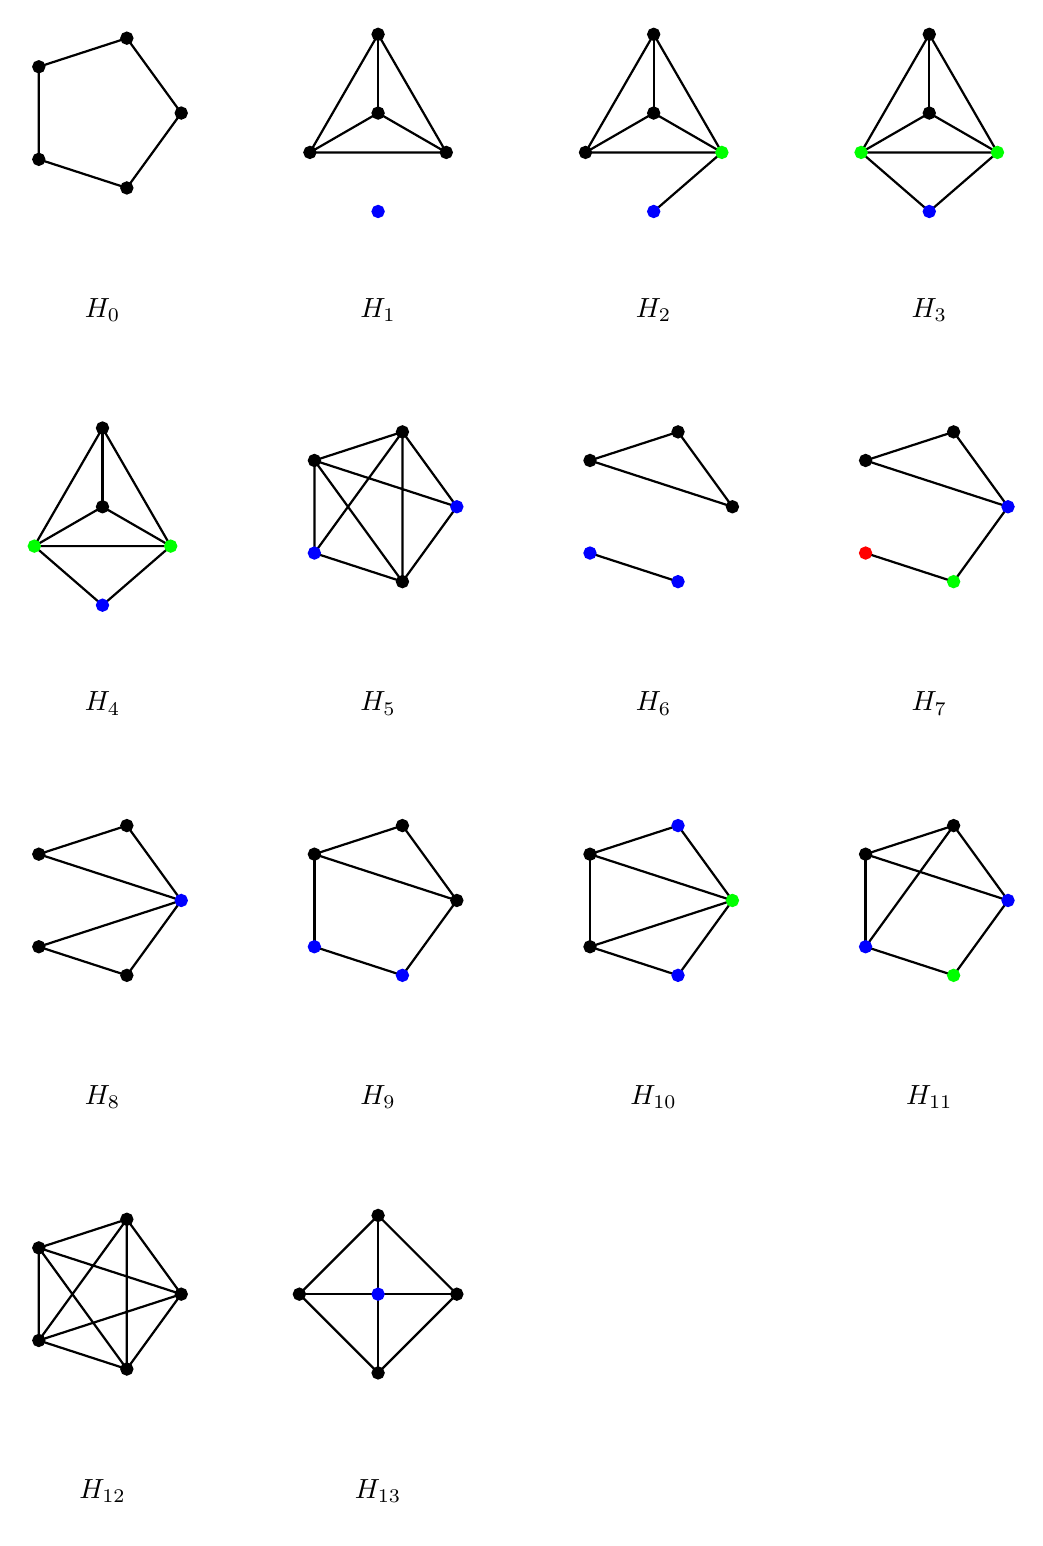
\begin{tikzpicture}[thick,scale=0.5]

% (0,0)
	\coordinate (center0_0) at (0:0);
	\coordinate (a1) at (0:2);
	\coordinate (a2) at (72:2);
	\coordinate (a3) at (144:2);
	\coordinate (a4) at (216:2);
	\coordinate (a5) at (288:2);
	\coordinate (lbl0_0) at (-90:5);
			
	\draw (a1) -- (a2) -- (a3) -- (a4) -- (a5) -- (a1);
	\draw (a2) node [color = black] {};
	\draw (a3) node [color = black] {};
	\draw (a4) node [color = black] {};
	\draw (a5) node [color = black] {};
	\draw (a1) node [color = black] {};
	\draw (lbl0_0) node [plain] {$H_0$};

	
% (0,1)
	\path (center0_0) ++ (0:7) coordinate (center0_1);

	\path (center0_1) ++ (-90: 2.5) coordinate (b1);
	\path (center0_1) ++ (0:0) coordinate (b2);
	\path (center0_1) ++ (90: 2) coordinate (b3);
	\path (center0_1) ++ (-30: 2) coordinate (b4);
	\path (center0_1) ++ (210: 2) coordinate (b5);
	\path (center0_1) ++ (-90:5) coordinate (lbl0_1);
	
	\draw (b5) -- (b3) -- (b4) -- (b5);
	\draw (b2) -- (b3);
	\draw (b2) -- (b4);
	\draw (b2) -- (b5);
	\draw (b1) node [color = blue]{};
	\draw (b2) node {};
	\draw (b3) node {};
	\draw (b4) node {};
	\draw (b5) node {};
	\draw (lbl0_1) node [plain] {$H_1$};


% (0,2)
	\path (center0_1) ++ (0:7) coordinate (center0_2);

	\path (center0_2) ++ (-90: 2.5) coordinate (c1);
	\path (center0_2) ++ (0:0) coordinate (c2);
	\path (center0_2) ++ (90: 2) coordinate (c3);
	\path (center0_2) ++ (-30: 2) coordinate (c4);
	\path (center0_2) ++ (210: 2) coordinate (c5);
	\path (center0_2) ++ (-90:5) coordinate (lbl0_2);
	
	\draw (c5) -- (c3) -- (c4) -- (c5);
	\draw (c2) -- (c3);
	\draw (c2) -- (c4);
	\draw (c2) -- (c5);
	\draw (c1) -- (c4);
	\draw (c1) node [color = blue]{};
	\draw (c2) node {};
	\draw (c3) node {};
	\draw (c4) node [color = green]{};
	\draw (c5) node {};
	\draw (lbl0_2) node [plain] {$H_2$};

% (0,3)
	\path (center0_2) ++ (0:7) coordinate (center0_3);

	\path (center0_3) ++ (-90: 2.5) coordinate (d1);
	\path (center0_3) ++ (0:0) coordinate (d2);
	\path (center0_3) ++ (90: 2) coordinate (d3);
	\path (center0_3) ++ (-30: 2) coordinate (d4);
	\path (center0_3) ++ (210: 2) coordinate (d5);
	\path (center0_3) ++ (-90:5) coordinate (lbl0_3);
	
	\draw (d5) -- (d3) -- (d4) -- (d5);
	\draw (d2) -- (d3);
	\draw (d2) -- (d4);
	\draw (d2) -- (d5);
	\draw (d1) -- (d4);
	\draw (d1) -- (d5);
	\draw (d1) node [color = blue]{};
	\draw (d2) node {};
	\draw (d3) node {};
	\draw (d4) node [color = green]{};
	\draw (d5) node [color = green]{};
	\draw (lbl0_3) node [plain] {$H_3$};


% (1,0)
	\path (center0_0) ++ (-90:10) coordinate (center1_0);

	\path (center1_0) ++ (-90: 2.5) coordinate (d1);
	\path (center1_0) ++ (0:0) coordinate (d2);
	\path (center1_0) ++ (90: 2) coordinate (d3);
	\path (center1_0) ++ (-30: 2) coordinate (d4);
	\path (center1_0) ++ (210: 2) coordinate (d5);
	\path (center1_0) ++ (-90:5) coordinate (lbl0_3);
	
	\draw (d5) -- (d3) -- (d4) -- (d5);
	\draw (d2) -- (d3);
	\draw (d2) -- (d4);
	\draw (d2) -- (d5);
	\draw (d1) -- (d4);
	\draw (d1) -- (d5);
	\draw (d1) node [color = blue]{};
	\draw (d2) node {};
	\draw (d3) node {};
	\draw (d4) node [color = green]{};
	\draw (d5) node [color = green]{};
	\draw (lbl0_3) node [plain] {$H_4$};

% (1,1)
	\path (center1_0) ++ (0:7) coordinate (center1_1);
	\path (center1_1) ++ (0:2) coordinate (e1);
	\path (center1_1) ++ (72:2) coordinate (e2);
	\path (center1_1) ++ (144:2) coordinate (e3);
	\path (center1_1) ++ (216:2) coordinate (e4);
	\path (center1_1) ++ (288:2) coordinate (e5);
	\path (center1_1) ++ (-90:5) coordinate (lbl1_1);
			
	\draw (e1) -- (e2) -- (e3) -- (e4) -- (e5) -- (e1) -- (e3) -- (e5) -- (e2) -- (e4);
	\draw (e2) node [color = black] {};
	\draw (e3) node [color = black] {};
	\draw (e4) node [color = blue] {};
	\draw (e5) node [color = black] {};
	\draw (e1) node [color = blue] {};
	\draw (lbl1_1) node [plain] {$H_5$};

% (1,2)
	\path (center1_1) ++ (0:7) coordinate (center1_2);
	\path (center1_2) ++ (0:2) coordinate (f1);
	\path (center1_2) ++ (72:2) coordinate (f2);
	\path (center1_2) ++ (144:2) coordinate (f3);
	\path (center1_2) ++ (216:2) coordinate (f4);
	\path (center1_2) ++ (288:2) coordinate (f5);
	\path (center1_2) ++ (-90:5) coordinate (lbl1_2);
			
	\draw (f1) -- (f2) -- (f3) -- (f1);
	\draw (f4) -- (f5);
	\draw (f2) node [] {};
	\draw (f3) node [] {};
	\draw (f4) node [color = blue] {};
	\draw (f5) node [color = blue] {};
	\draw (f1) node [] {};
	\draw (lbl1_2) node [plain] {$H_6$};

% (1,3)
	\path (center1_2) ++ (0:7) coordinate (center1_3);
	\path (center1_3) ++ (0:2) coordinate (g1);
	\path (center1_3) ++ (72:2) coordinate (g2);
	\path (center1_3) ++ (144:2) coordinate (g3);
	\path (center1_3) ++ (216:2) coordinate (g4);
	\path (center1_3) ++ (288:2) coordinate (g5);
	\path (center1_3) ++ (-90:5) coordinate (lbl1_3);
			
	\draw (g1) -- (g2) -- (g3) -- (g1);
	\draw (g4) -- (g5);
	\draw (g5) -- (g1);
	\draw (g2) node [] {};
	\draw (g3) node [] {};
	\draw (g4) node [color = red] {};
	\draw (g5) node [color = green] {};
	\draw (g1) node [color = blue] {};
	\draw (lbl1_3) node [plain] {$H_7$};


% (2,0)
	\path (center1_0) ++ (-90:10) coordinate (center2_0);
	\path (center2_0) ++ (0:2) coordinate (h1);
	\path (center2_0) ++ (72:2) coordinate (h2);
	\path (center2_0) ++ (144:2) coordinate (h3);
	\path (center2_0) ++ (216:2) coordinate (h4);
	\path (center2_0) ++ (288:2) coordinate (h5);
	\path (center2_0) ++ (-90:5) coordinate (lbl2_0);
			
	\draw (h1) -- (h2) -- (h3) -- (h1);
	\draw (h4) -- (h5) -- (h1) -- (h4);
	\draw (h2) node [] {};
	\draw (h3) node [] {};
	\draw (h4) node [] {};
	\draw (h5) node [] {};
	\draw (h1) node [color = blue] {};
	\draw (lbl2_0) node [plain] {$H_8$};

% (2,1)
	\path (center2_0) ++ (0:7) coordinate (center2_1);
	\path (center2_1) ++ (0:2) coordinate (i1);
	\path (center2_1) ++ (72:2) coordinate (i2);
	\path (center2_1) ++ (144:2) coordinate (i3);
	\path (center2_1) ++ (216:2) coordinate (i4);
	\path (center2_1) ++ (288:2) coordinate (i5);
	\path (center2_1) ++ (-90:5) coordinate (lbl2_1);
			
	\draw (i1) -- (i2) -- (i3) -- (i1);
	\draw (i4) -- (i5) -- (i1);
	\draw (i4) -- (i3);
	\draw (i2) node [] {};
	\draw (i3) node [] {};
	\draw (i4) node [color = blue] {};
	\draw (i5) node [color = blue] {};
	\draw (i1) node [] {};
	\draw (lbl2_1) node [plain] {$H_9$};

% (2,2)
	\path (center2_1) ++ (0:7) coordinate (center2_2);
	\path (center2_2) ++ (0:2) coordinate (j1);
	\path (center2_2) ++ (72:2) coordinate (j2);
	\path (center2_2) ++ (144:2) coordinate (j3);
	\path (center2_2) ++ (216:2) coordinate (j4);
	\path (center2_2) ++ (288:2) coordinate (j5);
	\path (center2_2) ++ (-90:5) coordinate (lbl2_2);
			
	\draw (j1) -- (j2) -- (j3) -- (j1);
	\draw (j4) -- (j5) -- (j1);
	\draw (j4) -- (j3);
	\draw (j4) -- (j1);
	\draw (j2) node [color = blue] {};
	\draw (j3) node [] {};
	\draw (j4) node [] {};
	\draw (j5) node [color = blue] {};
	\draw (j1) node [color = green] {};
	\draw (lbl2_2) node [plain] {$H_{10}$};

% (2,3)
	\path (center2_2) ++ (0:7) coordinate (center2_3);
	\path (center2_3) ++ (0:2) coordinate (k1);
	\path (center2_3) ++ (72:2) coordinate (k2);
	\path (center2_3) ++ (144:2) coordinate (k3);
	\path (center2_3) ++ (216:2) coordinate (k4);
	\path (center2_3) ++ (288:2) coordinate (k5);
	\path (center2_3) ++ (-90:5) coordinate (lbl2_3);
			
	\draw (k1) -- (k2) -- (k3) -- (k1);
	\draw (k4) -- (k5) -- (k1);
	\draw (k4) -- (k3);
	\draw (k4) -- (k2);
	\draw (k2) node [] {};
	\draw (k3) node [] {};
	\draw (k4) node [color = blue] {};
	\draw (k5) node [color = green] {};
	\draw (k1) node [color = blue] {};
	\draw (lbl2_3) node [plain] {$H_{11}$};

% (3,0)
	\path (center2_0) ++ (-90:10) coordinate (center3_0);
	\path (center3_0) ++ (0:2) coordinate (l1);
	\path (center3_0) ++ (72:2) coordinate (l2);
	\path (center3_0) ++ (144:2) coordinate (l3);
	\path (center3_0) ++ (216:2) coordinate (l4);
	\path (center3_0) ++ (288:2) coordinate (l5);
	\path (center3_0) ++ (-90:5) coordinate (lbl3_0);
			
	\draw (l1) -- (l2) -- (l3) -- (l4) -- (l5) -- (l1) -- (l3) -- (l5) -- (l2) -- (l4) -- (l1);
	\draw (l2) node [] {};
	\draw (l3) node [] {};
	\draw (l4) node [] {};
	\draw (l5) node [] {};
	\draw (l1) node [] {};
	\draw (lbl3_0) node [plain] {$H_{12}$};

% (3,1)
	\path (center3_0) ++ (0:7) coordinate (center3_1);
	\path (center3_1) ++ (0:0) coordinate (m1);
	\path (center3_1) ++ (90:2) coordinate (m2);
	\path (center3_1) ++ (180:2) coordinate (m3);
	\path (center3_1) ++ (-90:2) coordinate (m4);
	\path (center3_1) ++ (0:2) coordinate (m5);
	\path (center3_1) ++ (-90:5) coordinate (lbl3_1);
			
	\draw (m2) -- (m3) -- (m4) -- (m5) -- (m2);
	\draw (m1) -- (m2);
	\draw (m1) -- (m3);
	\draw (m1) -- (m4);
	\draw (m1) -- (m5);
	\draw (m2) node [] {};
	\draw (m3) node [] {};
	\draw (m4) node [] {};
	\draw (m5) node [] {};
	\draw (m1) node [color = blue] {};
	\draw (lbl3_1) node [plain] {$H_{13}$};



\end{tikzpicture}


In each of the above drawings, we name the set of black vertices $\mathcal{O}_0$, the blue vertices  $\mathcal{O}_1$, the green vertices $\mathcal{O}_2$, and the red vertices $\mathcal{O}_3$.

Suppose that $G_c$ is graph on $n$ vertices with $\nu_c(G_c) \leq n/c$.  Define a function $\# : [13] \cup {0} \times [3] \rightarrow \mathbb{N}$ so that $\#(i,j)$ is  the minimum number of distinct copies of $H_i$ in which a vertex $v \in V(G)$ appears as a member of orbit $\mathcal{O}_j$ (when defined, otherwise 0). 

\begin{theorem}
	For any $0 \leq i \leq 13$, if $G$ is a  \kfree graph on $n$ vertices with some vertex not in an induced subgraph isomorphic to $H_i$, then $G$ has a connected matching of size at least $\lfloor n/c \rfloor$ ($c$ to be determined later, for sure $c\leq 16$).
\end{theorem}

\begin{proof}
	\begin{description}
		\item
		\item[$H_0$:] The neighborhood of any vertex must induce some non edge (otw large clique).  Let $v_1$ and $v_2$ be non adjacent nieghbors of some vertex $v$.  Let $S = N(v_1) \cap \overline{N(v)}$ and $T = N(v_2) \cap \overline{N(v)}$.  If there is no induced $C_5$ including $v$ in $G$, then one of $S \Delta T \cap S$ or  $S \Delta T \cap T$ is empty.  Hence, either $S\subset T$ or $T\subset S$.  Since $G$ is \kfree, $S \cup T  = \overline{N(v)}$.  Hence one of $vv_1$ or $vv_2$ is a dominating edge, and we can carry out an induction step (HC2-strong).  
		\item[$H_1$:] If any vertex has degree greater than $n-c-1$ we can carry out an inductive step.
		\item[$H_2$] Work on green vertex.  If neighborhood complement has max degree 2, then the neighborhood has a large clique.
		\item[$H_3$] \sout{Must exist an edge disconnected from a vertex.  If no edge from said vertex into intersection of endpoint nbds, then this is a large clique}???
		\item[$H_4$] Oops, thats the same as $H_3$.
		\item[$H_5$] If two non-adjacent vertices have nbds with small intersection, then there is a large clique
		\item[$H_6$] Kriesell showed HC2-strong.  Simpler proof for this weaker result- if  $v\notin H_6$, $v$ is in a dominating edge.
		\item[$H_7$] Must be non-edges in nbd, if max deg from nbd to non nbd is 2, max non-deg is 4.
		\item[$H_8$] Nbd induces no $2K_2$ $\implies$ near perfect conn match (in nbd)
		\item[$H_9$] edges from endpoints of a non-edge in the nbd to the non-nbd either totally coincide and dominate ($\implies$ dominating edge) or are distinct and cover it. ...implies perfection of nbd, but is tricky
		\item[$H_{10}$] If nbd is $P_4$-free it is perfect.
		\item[$H_{11}$] Again with the tricky implication of perfection of nbd
		\item[$H_{12}$] max degree issue
		\item[$H_{13}$] $\{\overline{K_3}, P_4\}$-free graph decomposes into three cliques.  $P_4$-free nbd has a large clique 
	\end{description}
\end{proof}

\end{document}